\section{Current}
Current$(i)$ is the force that moves charge through a circuit. Current can be defined as an amount of charge moved over a time interval. This can be expressed as the following relation: \cite[p.~3]{bcircuit5}
\begin{align}
i(t)=\dfrac{dq(t)}{dt} \Leftrightarrow q(t)=\int i(t)\ dt,\label{I=dq/dt}
\end{align}
where $i(t)$ is the current (in ampere, $A$) at a given time $t$ (in seconds, $s$), and $q(t)$ is the function for charge at a given time $t$. $q(t)$ is measured in coulomb $(C)$.
\\
There exist two types of current: alternating current (AC) and direct current (DC). Per definition, DC current is a constant flow of current, while AC alternates (see figure \ref{fig:ACDC}). 
\begin{figure}[H] 
\begin{tikzpicture}
\begin{axis}[ticks=none,
axis lines =center,
xlabel={t},
ylabel={i(t)},
    height=7cm, width=9cm,
    xmin=0, xmax=10, ymin=-2, ymax=2]
\addplot [
    domain=0:10, 
    samples=100, 
    color=red,
]
{1};
\addlegendentry{$DC$}
\addplot [
    domain=0:10, 
    samples=100, 
    color=blue,
    ]
    {sin(\x r)};
\addlegendentry{$AC$}
\end{axis}
\end{tikzpicture}
\caption{AC and DC versus time}
\label{fig:ACDC}
\end{figure}
\noindent
A sinusoidal AC current can be described with the function: 
\begin{align}
i\left(t, f, A, \theta\right) =& A\cdot \sin{\left(2\pi ft + \theta\right)}, \nonumber
\\
=& A \cdot \sin{\left(\omega t + \theta\right)}, \label{eq:omega}
\end{align}
where $f$ is frequency (in hertz, $Hz$), which is cycles per second, $\omega = 2\pi f$ (in radians per second, $s^{-1}$), $t$ is time (in seconds, $s$), $A$ is amplitude (in ampere, $A$), and $\theta$ is the phase shift (in radians, unit-less).
For ease of understanding, $\omega$ is sometimes used for notation instead of $2\pi f$. $\omega$ is also called the angular frequency of the signal.
This function can be plotted as such:
\begin{figure}[H]
	\centering
	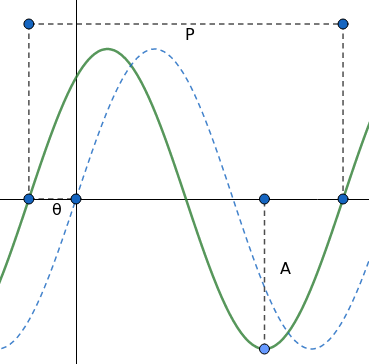
\includegraphics[scale=0.7]{fig/img/AC.png}
	\caption{Two AC currents, $i(t)=A\sin(\omega t)$ and $i(t)=A\sin(\omega t+\theta)$ shown in dotted blue line and green respectively. The 'green' current has been phase shifted by $\theta$. The currents have amplitude $A$, and period $P=f^{-1}$.}
\end{figure}
\noindent A certain type of AC exists where the current is constant for a half period and then turned off for half period. This kind of AC is called a step voltage.
\begin{figure}[H] 
\begin{center}
\begin{tikzpicture}
\begin{axis}[ticks=none,
axis lines =center,
xlabel={t},
ylabel={i(t)},
    height=7cm, width=9cm,
    xmin=0, xmax=10, ymin=-2, ymax=2]
\addplot [
    domain=0:3.14, 
    samples=100, 
    color=red,
]
{1};
\addplot +[mark=none, color=red] coordinates {(3.14, 0) (3.14, 1)};
\addplot [
    domain=3.14:6.28, 
    samples=100, 
    color=red,
    ]
    {0)};
\addplot +[mark=none, color=red] coordinates {(2*3.14, 0) (2*3.14, 1)};
\addplot [
    domain=6.28:9.42, 
    samples=100, 
    color=red,
]
{1};
\addlegendentry{AC step input}
\end{axis}
\end{tikzpicture}
\end{center}
\caption{Current for AC step input}
\end{figure}
\section{Voltage}
Voltage ($v$), also called electric potential difference, is the change in potential energy that a charge undergoes, when it passes through two given points in a circuit. This is expressed in the following equation:
\begin{align*}
	v=\dfrac{dU(q)}{dq},
\end{align*}
\\
where $U(q)$ is the function for potential energy (in joules, $J$), given a charge $q$.
\section{Resistor}
When a resistor, which is a passive element, is added to a circuit, it creates a resistance($R$). Resistance makes it more difficult for the current to pass through the element. Resistance is defined as the proportional constant between current and voltage. The mathematical relation of this is given by: \cite[p.~22]{bcircuit5}
\begin{align} 
\label{Ohm}
v(t)=R\cdot i(t),\ R\geq0,
\end{align}
where $R$ is resistance (in Ohm, $\Omega$).
\section{Power} 
Power ($p$) measures the effect (in watts, $W$). Power can be expressed as: \cite[p. 22]{bcircuit5}.
\begin{align} 
\label{power}
p(t)=v(t)\cdot i(t).
\end{align}
By inserting this in equation \eqref{Ohm}, the following expression is found:
\begin{align}
p(t)=\dfrac{v^2(t)}{R}. \label{resistor:power}
\end{align}
This is defined as the amount of work done per time. 
\section{Capacitor}
A capacitor, which is a passive element, consists of two similar sized plates. When a current is applied to the circuit, the capacitor gets charged. The capacitance($C$) is the amount of energy a capacitor can store, when it is fully charged. The capacitor gets charged, when a positive charge is transferred from one plate to another through the circuit.
\\
The capacitance is given by the following equation:
\begin{align*}
C=\dfrac{\epsilon_{0}A}{d},
\end{align*}
where $C$ is the capacitance (in farad, $F$) and $\epsilon_{0}$ is the permittivity of free space, which is equal to $8.85 \cdot 10^{-12}                                                 \frac{F}{m}$. $A$ is the surface area of the plates (in square meters, $m^{2}$), and $d$ is the distance between the two plates (in meters, $m$).
\\
The charge of a capacitor across a voltage ($v$) and capacitance ($C$) is equal to: \cite[p.~253]{bcircuit5}
\begin{align}
\label{QCV}
q_C(t) = Cv_C(t).	
\end{align}
From \eqref{I=dq/dt}, current is defined as:
\begin{align*}
	i(t) = \frac{dq(t)}{dt}.
\end{align*}
The current across a capacitor is then:
\begin{align*}
	i_C(t) = \frac{d}{dt}\big(Cv_C(t)\big).
\end{align*}
For a capacitor with capacitance ($C$), the current through the capacitor can be written as:
\begin{align}
	i_C(t) = C\frac{dv_C(t)}{dt}.\label{iC}
\end{align}
\section{Time constant}
A constant that shows up when looking at RC circuits, is the time constant $\tau = R \cdot C$, where $R$ is the resistance of the resistor, $C$ is the capacitance of the capacitor, and $\tau$ is time (in seconds, $s$).

% Forslag til første sætning:
% The product of the resistance and capacitance is a useful time constant when looking at RC circuits.